\documentclass[10pt,twocolumn,a4paper]{article}
\usepackage[margin=18mm,columnsep=6mm]{geometry}
\usepackage{amsmath,amssymb,booktabs,microtype,graphicx,tikz,pgfplots}
\usepackage[hidelinks]{hyperref}
\usepackage{xurl,placeins}
\pgfplotsset{compat=1.18}
\setlength{\emergencystretch}{1em}
\newsavebox{\databox}
\renewcommand{\dbltopfraction}{.9}
\renewcommand{\textfraction}{.1}
\title{Digital-Twin-Guided Predictive Autoscaling:\\Capacity Calibration, Ready Reserves and Repeated Kubernetes Evaluation}
\author{Shehryar Faisal \and Abdul Mahid \and Basharat Hussain}
\date{November 2026}
\renewcommand{\dbltopfraction}{0.95}
\renewcommand{\dblfloatpagefraction}{0.85}
\renewcommand{\textfraction}{0.05}
\begin{document}
\twocolumn[\begin{@twocolumnfalse}\maketitle
\begin{abstract}
We reproduced a published Prophet--LSTM forecaster, then tested how many ready replicas a service would need to meet a request latency objective. Our first controller often missed that objective. In some decisions, its latency-error margin alone exceeded the target, leaving no replica count that could satisfy the model. Fixed deployments also ran short of capacity during peak load. The revised controller uses a capacity threshold measured in load tests, recent CPU cost and an upper demand estimate to size the deployment. It keeps a reserve of ready replicas and delays scale-down after pressure.

On a local K3s cluster, 75 primary trials produced 120275 measured requests. The revised controller met the objective of at least 99\% HTTP-200 responses within 500 ms in all 15 workload--seed cells; the original dual policy met it in none and CPU HPA in one. Mean trial violation rates were 0.00\%, 19.82\% and 31.65\%, respectively. Mean desired allocation was 27.99 pod-minutes for the revision and 34.18 for fixed sixteen-replica capacity. However, eighteen additional trials with the same minimum of eight replicas showed that native HPA also met the objective in all nine cells, using 17.09 mean pod-minutes against 28.07 for the revision. We also checked response predictions in eighteen live validation blocks and tested controller variants in 1,000 simulation rollouts. The live comparison supports the changes to our initial controller and leaves any advantage over HPA with the same reserve unproven. Code and experimental artifacts are available at \url{https://github.com/shehryarf67/uncertainty-aware-digital-twin-k8s-autoscaling}.

\end{abstract}\vspace{4mm}\end{@twocolumnfalse}]


\section{Introduction}
A workload forecast estimates how many requests will arrive. An autoscaler must also decide how many replicas can serve those requests within the required response time, and when those replicas must be ready. These decisions depend on request cost and startup delay as well as demand. Studies of Kubernetes HPA operation and tuning show why resource settings matter when evaluating a scaling policy \cite{j01,j02}.

We began with the Prophet--LSTM method of Guruge and Priyadarshana \cite{guruge}. Reproducing its released code and then evaluating a separate causal implementation gave us two different views of forecasting accuracy. Neither evaluation measured whether a running application could meet a request-latency objective. We therefore implemented a service-response model and tested the resulting scaling decisions on Kubernetes.

The first controller exposed a problem in how prediction error was used. In twelve of 48 dual-policy decisions, the latency correction alone exceeded the 500-ms target. Adding capacity could not make any positive predicted latency satisfy that surrogate constraint. Development load tests also showed failures with fixed six-replica capacity at peak conditions on the host. These observations motivated changes to both sizing and the capacity limit.

The revised implementation sizes replicas using a measured capacity envelope and recent request CPU cost. It keeps ready capacity available while additional pods start, and delays scale-down after observed pressure. We evaluate the combined revision against the original dual policy, a reserve ablation, native CPU HPA and fixed capacity. Raising the maximum from six to sixteen replicas changes the experimental conditions, so we rerun the original policy under the expanded limit instead of attributing the entire pilot-to-revision difference to the algorithm.

We use the forecasting traces to ask how much the reported error changes when each prediction uses only observations available at its issue time. On the cluster, our outcomes are SLO compliance and desired pod-minutes. Comparing policies at the same minimum replica count and switching off individual controller rules helps us examine which parts of the design contributed to those outcomes.

\section{Related Work}
Guruge and Priyadarshana add an LSTM residual estimate to Prophet's trend and seasonal forecast \cite{guruge,prophet,lstm}. That architecture belongs to the trace experiments. On the cluster, a separate predictor works from recent request counts, so better trace RMSE would not in itself explain a live SLO result.

Autoscaling surveys cover provisioning across cloud, container, edge and IoT systems \cite{j06,j08,j09,j24,j26}. For our Kubernetes comparison, the relevant point is where a policy changes the control loop. CPU HPA has tunable targets and replica bounds \cite{j01,j02}. SATA adjusts the target in response to service-level behaviour \cite{j04}, while Mondal et al.\ implement workload prediction and replica evaluation through the Custom Pod Autoscaler framework \cite{j03}. Our first comparison changed both the controller and the minimum replica count. We matched the minimum in a separate experiment to see how native HPA performed with the same floor.

Predictive container methods include bidirectional LSTM and attention-based GRU encoder--decoder models \cite{j18,j05}. K-AGRUED also considers cooldown and conflicting scaling actions \cite{j05}; readiness and actuation timing are therefore existing concerns rather than a new problem introduced by our study. Informer, transformer and SCINet approaches provide further forecasting alternatives \cite{j13,j15,j25}. Related cloud workload studies examine predictor combinations, multiple time series, nonstationary patterns and forecast-output processing \cite{j16,j22,j23,j29}. We do not implement these alternatives, so the experiments cannot rank our controller against them.

Adaptive containers, bio-inspired control, online VM scaling, multi-resource prediction and dynamic-workload scaling address other parts of resource management \cite{j07,j10,j11,j14,j17}. Work on allocation transitions and formal verification further distinguishes making a scaling recommendation from executing or verifying it \cite{j12,j27}. Here we measure actual request outcomes and sample desired and ready replicas separately to examine the consequences of execution delay.

Digital-twin reference models and surveys describe broader synchronization between a system and its virtual representation \cite{j19,j28}. Our response model covers only a conditional relation between offered CPU work, replica count and tail latency. Likewise, conformal multi-step forecasting methods study prediction intervals under their own constructions and assumptions \cite{j20,j21}. Our forty-score correction has no inherited 99\% coverage theorem. The research question is therefore whether these specific implementation choices help in the recorded workload cells, with their resource costs and failure cases reported alongside successful outcomes.

\section{Baseline Validation}
Let $y_t$ be workload, $p_t$ a Prophet estimate and $r_t=y_t-p_t$ its residual. A causal one-minute hybrid predicts
\begin{equation}\widehat y_{t\mid t-1}=p_t+f_\theta(r_{t-1}).\end{equation}
For target $t$, the LSTM receives the preceding residual rather than the residual of the observation being scored. Once a test observation has occurred, it may be used for the next forecast. This gives a rolling one-step evaluation, rather than a forecast of the entire test period from a single origin. The official supplied NASA-HTTP and WorldCup98 files contain 81,396 and 125,300 observed minute rows, with chronological 70/30 partitions of 56,977/24,419 and 87,710/37,590. They omit 7,884 and ten calendar minutes. Gap filtering leaves 24,390 NASA and 37,590 WorldCup eligible targets; missing traffic is not asserted to be zero.

The NASA notebook fits linear Prophet growth and the WorldCup notebook fits flat growth. They share a changepoint prior of 5.1 and seasonality prior of 30, with Fourier orders of 50 for daily and 20 for weekly seasonality. Yearly seasonality is disabled. In both notebooks, one residual enters two 50-unit LSTM layers and a linear output layer. Training uses Adam and MSE, with batches of 16 and a validation fraction of 0.2. The notebooks allow 20 epochs and the paper reports 50. In our four faithful fits, the five-epoch patience rule stopped training at epoch six and restored the first epoch's weights. We ran two fits per trace on an Intel i7-1255U using Python 3.12.14, TensorFlow 2.17, Keras 3.4.1 and Prophet 1.1.5.

Consider a residual from row $i$. The released notebook uses it to predict row $i+1$, then puts that prediction back on row $i$. The final row has no aligned prediction and is filled with its observed residual, yielding an exact final prediction. In NASA, the scaler sees all residuals. In WorldCup, the count scaler is fitted before the split. We keep those details in the faithful runs. The causal implementation moves the prediction to its target row, drops the final-row fallback, excludes targets across gaps and fits the transforms on the early neural training prefix. Random states are fixed to 42. Prophet fits the full outer training period, so neural validation uses residuals conditional on that Prophet fit. Outer-test observations stay outside all fitting.


\begin{table}[t]\centering\small\setlength{\tabcolsep}{3pt}
\caption{Forecast RMSE. Faithful means use full released tests; causal NASA excludes 29 gap targets. WorldCup is displayed on the common author scale after causal fitting.}\label{tab:baseline}
\savebox{\databox}{%
\begin{tabular}{lrrr}\toprule
Trace & Published & Faithful & Causal\\\midrule
NASA & 7.990 & 8.02163 & 14.2902\\
WorldCup & 0.003358 & 0.00337950 & 0.00388174\\
\bottomrule\end{tabular}
}
\ifdim\wd\databox>\columnwidth\relax\resizebox{\columnwidth}{!}{\usebox{\databox}}\else\usebox{\databox}\fi
\end{table}


On common NASA targets, faithful mean RMSE is 8.01251. WorldCup causal raw-count RMSE is 890.5685, compared with persistence at 762.7463; NASA persistence is 16.3871. The causal WorldCup hybrid therefore has a higher raw-count RMSE than persistence in this evaluation. NASA shows the opposite ordering against persistence. Because alignment, scaling and gap handling were corrected together, the change from faithful to causal scores cannot be assigned to one correction. The saved predictions and model files allow both evaluations to be inspected.

\section{Initial Controller Diagnosis}
An earlier integration check connected the authors' Java 21/Spring Boot 3.4.2 application and forecasting scaler to KEDA 2.18, Prometheus 2.55.1 and local K3s. Scaler logic was preserved while compatible gRPC bindings were regenerated. Stable, increasing, spike and decreasing scenarios produced 6,870 measured requests per controller in scheduling-validated runs. Forecast KEDA and CPU HPA had zero HTTP failures and zero observations above 500 ms. Forecast scaling held three replicas; HPA moved from one to three. Sampled allocation was 23.286 versus 13.778 pod-minutes. The integration test confirmed that the scaler could issue decisions through KEDA and that the application served the offered traffic. Since both policies stayed within the latency threshold, it supplied little evidence about how either policy would behave near overload.

For the next tests, we needed a service that could saturate on the local host. We used a CPU-bound application and fitted the pilot's monotone response curve $g(x)$ to effective P99. Its input $x=\lambda c/n$ is the offered request rate times the median CPU milliseconds per request, divided by the number of ready replicas. Eighteen blocks fit the curve and twelve calibrate the latency margin. The dual policy adds margins for demand and latency, looks ahead two cycles, and checks replica counts from one to six. Each cycle offers traffic for five seconds and gives outstanding requests another three seconds to drain.

The pilot archive contains fifteen trials. Across its three repetitions, the dual policy averaged 10.40\% request violations and met the SLO once. The point-only Twin averaged 39.67\%. In the dual-policy logs, 12 of 48 decisions had a latency margin above 500 ms before the model added any predicted latency. Every candidate then failed the check and the code fell back to six replicas. A residual measured while requests queue at the current replica count can therefore disqualify a larger deployment too. We addressed that failure by sizing from CPU work per ready replica measured in fixed-capacity tests.

\section{Controller Revision}
\subsection{Objective and Capacity Evidence}
A request complies only if HTTP status is 200 and measured client latency $\ell_i\leq500$ ms. The request objective is
\begin{equation}v=\frac{1}{N}\sum_i\mathbf1\{\mathrm{status}_i\ne200\lor\ell_i>500\mathrm{\ ms}\}\leq0.01.\label{eq:slo}\end{equation}
The scorer checks status as well as latency, so a fast error or a timeout counts as a violation. To calculate desired pod-minutes, we multiply each sampled desired count by the time it remains in effect and sum over the trial. Requested replicas contribute while they are becoming ready.

The revised experiments use that same PBKDF2 service. Each pod requests 250m CPU and 96Mi memory, with limits of 500m and 192Mi. A semaphore permits one processing task per pod. A request that waits more than two seconds for admission receives HTTP 429; the client timeout is three seconds. Pods wait five seconds at startup and are checked for readiness every two seconds. CPU limits can lead to throttling \cite{j01,j12}. This service is separate from the original authors' application, whose source and forecasting baseline remain preserved.

We profiled fixed deployments of 4, 6, 8, 12 and 16 replicas. For each size, we offered 5, 25 and 45 requests/s at unit work and 30 requests/s at 1.8 times unit work. The 4--12 replica blocks ran traffic for five seconds and drained for three. The sixteen-replica blocks offered traffic for fifteen seconds. Across the twenty blocks we measured 3,675 requests. The six-replica deployment missed the SLO at both 45 requests/s and the higher work setting. We saw no violations in the longer sixteen-replica blocks and chose sixteen as the common ceiling for the policy comparison.

For block $j$, we compute $x_j=\lambda_jc_j/n_j$ and fit the monotone curve to effective P99. In that diagnostic, a failed response gets a penalty of at least 2,000 ms. Client quantiles still use measured latency, and Equation~\ref{eq:slo} uses both the measured latency and status. We derive the sizing threshold from the same development profile:
\begin{align}
\mathcal A&=\{j:v_j\leq0.01,\ P99_j\leq400\mathrm{\ ms}\},\\
C&=\min\{200,\ 0.8\max_{j\in\mathcal A}x_j\}.\label{eq:capacity}
\end{align}
The screening step selects development conditions that passed both the request objective and a stricter 400-ms P99 check. We then leave 20\% headroom and cap the threshold at 200 CPU-ms/s per ready replica. These settings were fixed before evaluation. In the implementation, this threshold drives sizing; the fitted response curve supplies a predicted tail value and a support diagnostic. Neither operation certifies future latency compliance.

\subsection{Demand and Cost Corrections}
At each decision, the harness provides the observed arrival count, completed-response measurements, and desired and ready replica counts. Two five-RPS warm-up cycles initialize the rate history and provide an initial P90 CPU cost from successful responses. Thereafter, the controller keeps the latest four available CPU-P90 estimates and uses their maximum, $\bar c_t$. An estimate above the current maximum raises the sizing input immediately. Lower estimates reduce it only after the higher values leave the window.

The controller starts from the largest rate in the latest three observations. It also projects the current rate forward by adding $h_t$ times the last nonnegative rate increase. The larger value becomes $\widehat\lambda_t$. When the $h_t$ observations for that forecast are available, the controller scores it as their maximum minus the forecast it issued. It keeps up to forty of those errors. At nominal 99\%, the rank used by the code selects the largest available error. The correction $q_t$ is that error if positive, and zero when the buffer is empty or its maximum is nonpositive. We evaluate coverage empirically. This rule does not provide an exact distribution-free 99\% guarantee.

\subsection{Readiness, Pressure and Scale-Down}
When a scale-up is issued, the controller stores its time and target. Once the observed ready count reaches that tracked target, it updates the startup estimate by averaging the previous estimate with the elapsed time, subject to an eight-second floor. The planning horizon is
\begin{equation}h_t=\max\{2,\min(6,\lceil\widehat d_t/8\rceil+1)\}.\end{equation}
The nominal startup estimate is eight seconds. At each completed observation, the provisional replica requirement is
\begin{equation}n_t^{\rm req}=\left\lceil\frac{(\widehat\lambda_t+q_t)\bar c_t}{C\beta_t}\right\rceil+2,\label{eq:sizing}\end{equation}
clipped to the common maximum, with an eight-replica desired reserve initialized with all eight ready. The two additional replicas and reserve are explicit resource costs. The reserve ablation removes only the eight-replica floor; it begins with the same eight ready replicas and retains the other logic.

The factor $\beta_t\in[0.5,1]$ reduces the usable capacity threshold after pressure is observed. If violations exceed 0.5\% or effective P99 exceeds 450 ms, the code multiplies it by 0.85, down to a floor of 0.5. After eight clean observations, it increases by 0.025 per cycle until it reaches one. Crossing either pressure threshold also starts a three-cycle hold at the maximum replica count, including the current cycle. The emergency branch requests that maximum if the hold is active, the violation rate exceeds 1\%, or effective P99 exceeds 500 ms.

Before removing a replica, the code checks two counters. It needs three consecutive recommendations below the current desired count and at least three clean observations. The current deployment must also have as many ready replicas as desired, with cumulative violations at or below 0.5\%. If those checks pass, the controller drops at most one replica at that decision.

The controller logs the predicted P99 and a feasibility flag alongside the requested count. The flag checks the upper end of the measured work range, a predicted P99 of at most 500 ms, and whether the raw replica requirement fits under the limit. SLO compliance is calculated separately from observed requests using Equation~\ref{eq:slo}.

\begin{figure}[t]\centering
\resizebox{\columnwidth}{!}{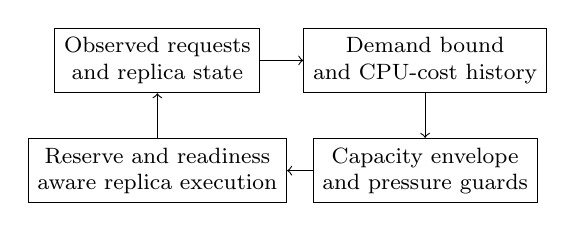
\begin{tikzpicture}[font=\footnotesize]
\node[draw,align=center] (o) at (0,0) {Observed requests\\and replica state};
\node[draw,align=center] (p) at (3.4,0) {Demand bound\\and CPU-cost history};
\node[draw,align=center] (t) at (3.4,-1.4) {Capacity envelope\\and pressure guards};
\node[draw,align=center] (a) at (0,-1.4) {Reserve and readiness\\aware replica execution};
\draw[->] (o)--(p);\draw[->] (p)--(t);\draw[->] (t)--(a);\draw[->] (a)--(o);
\end{tikzpicture}}
\caption{Implemented revision. Decisions use only observed telemetry; future traffic and work schedules remain confined to the load generator.}\label{fig:architecture}\end{figure}

\section{Experimental Design}
\subsection{Repeated Kubernetes Evaluation}
We run the expanded study on the same local Intel host, using K3s v1.33.6+k3s1 and containerd 2.1.5 under Ubuntu WSL2. The external controller reaches the Kubernetes API through a loopback-only proxy. The frozen protocol records hashes of the controller, harness and development inputs, so the analysis can check whether the evaluated source changed.

We compare guarded control, the original dual policy, the reserve ablation, CPU HPA and a fixed deployment of sixteen replicas. The dual policy reads its pilot profile and runs its original decision logic with the limit raised to sixteen. We wait for eight ready replicas before starting any adaptive policy. The fixed deployment starts with sixteen. The harness excludes setup and two warm-up cycles from both the request and allocation totals.

After warm-up, the harness installs CPU HPA with a 70\% target relative to CPU requests and a range of one to sixteen replicas. It uses zero seconds of scale-up stabilization and 24 seconds of scale-down stabilization. HPA reconciles on its native schedule \cite{j01}. The external controller processes observations every eight seconds. The comparison therefore includes the effects of their different feedback timing.

The primary study uses seeds 404, 505, 606, 707 and 808. Each seed determines the order of the scenarios and policies. We fixed the three sixteen-cycle workloads before final testing (Table~\ref{tab:workloads}). One repeats the pilot batch pattern. The two new patterns introduce abrupt changes and uninterrupted traffic, respectively. Only the load generator sees the future rates and work multipliers.

In the primary comparison, HPA can fall to one replica and guarded control keeps at least eight. After inspecting early primary outcomes, we specified a separate exploratory comparison that gives both policies the same range of eight to sixteen replicas. Seeds 909, 1010 and 1111 give eighteen trials on the same workloads, with the scenario and policy order shuffled within each seed. We used the frozen guarded controller for these trials.


\begin{table*}[t]\centering\small\setlength{\tabcolsep}{3pt}
\caption{Each cycle spans eight seconds. Batch workloads offer traffic for five seconds and pause for three; continuous traffic uses all eight. Work multipliers rise to 1.8 in cycles 13--16 of the previous batch, to 1.6 in cycles 11--13 of abrupt batch, and to 1.6 in cycles 11--16 of continuous traffic. Other cycles use unit work.}\label{tab:workloads}
\savebox{\databox}{%
\begin{tabular}{lrrl}\toprule
Workload & Active s/cycle & Requests/trial & Rate sequence (requests/s)\\\midrule
Previous batch & 5 & 1400 & 5, 5, 5, 5, 10, 15, 20, 25, 45, 45, 15, 10, 25, 30, 15, 5\\
Abrupt batch & 5 & 1315 & 5, 5, 5, 5, 40, 40, 40, 8, 8, 8, 28, 28, 28, 5, 5, 5\\
Continuous & 8 & 2096 & 6, 6, 9, 15, 22, 32, 40, 18, 8, 5, 25, 30, 18, 8, 15, 5\\
\bottomrule\end{tabular}
}
\ifdim\wd\databox>\textwidth\relax\resizebox{\textwidth}{!}{\usebox{\databox}}\else\usebox{\databox}\fi
\end{table*}


The generator uses absolute send deadlines, jittered request slots and no connection reuse. The harness runs traffic generation, replica sampling and control as separate tasks. In the continuous workload, time spent querying or updating the API therefore does not intentionally pause the send schedule. Recorded dispatch delays provide a check on whether the generator kept up. Requests retain send/finish times, HTTP status, latency, CPU and queue information where observed, and dispatch delay. Every scheduled request enters final scoring, including late completions and timeouts. Control feedback at a boundary uses completed outcomes before that boundary and outstanding-response ages, with no future response payloads.

A monitor reads desired and ready counts about once per second. The harness integrates desired allocation through the end of the trial. The archive lets us bound the contribution after the final sample because it retains the sample times but omits the exact end clock. A trial must complete, record one decision observation per cycle, send the expected number of requests and have zero sampler errors. Maximum dispatch delay, sampler gap and decision lateness must be below 500 ms, three seconds and one second, respectively. The protocol allows one retry for timing-invalid runs and stores both attempts. An SLO miss alone does not trigger a retry.

\subsection{Historical Bounds and Independent Plant}
For the historical bound analysis, we reuse saved causal forecasts and do not retrain the predictors. We take the first 20\% of eligible outer-test targets as a new calibration prefix: 4,878 NASA observations and 7,518 WorldCup observations. This leaves 19,512 and 30,072 targets for evaluation. The static correction uses the prefix's upper-error quantile. The adaptive correction starts from its last forty errors and updates after each new outcome. This analysis measures how often the demand stays below an upper bound; it does not test application response time.

To check the fitted response mapping, we measure eighteen combinations outside the development set: 6, 10 and 14 replicas crossed with 12, 24 and 36 requests/s and work multipliers of 1.1 and 1.5. Each block offers traffic for five seconds and allows three seconds for drainage, for 2,160 requests in total. The curve and capacity threshold remain frozen. The input CPU cost is measured within each block. The check therefore concerns response prediction conditional on realized cost, rather than the ability to predict a future change in CPU demand.

The simulation uses a separate queueing plant to generate response outcomes. Arrivals follow a Poisson process and request CPU work is lognormal, with log-scale standard deviation 0.3. Mean unit-work cost comes from the development measurements. A central dispatcher assigns each arrival to the earliest free ready server, which supplies 0.5 CPU core. The plant models queue admission and the three-second client timeout. CPU work becomes visible to the controller only through successful completed responses. Outcomes assigned to a removed server still enter scoring. The fitted response curve is not used to generate these labels.

Twenty-five paired seeds, five regimes and eight policies give 1,000 rollouts of 64 eight-second cycles. Regimes cover smooth demand, bursts, a 1.8-fold service-cost shift, startup delay increased from eight to 24 seconds, and one-cycle observation delay. In the delay case, demand, response and CPU feedback are delayed while replica state remains current. Policies include the guarded revision, reserve ablation, original dual policy, CPU-reactive proxy, fixed eight and fixed sixteen replicas, and isolated emergency-response and horizon ablations. The latter change only the named assignment in the frozen controller method. The proxy is not native HPA. Shared arrival/service input hashes verify pairing across policies.

\subsection{Analysis and Claim Scope}
We first assess each trial against the request objective, then summarize compliance counts by workload. Violation percentages, P99 values and desired allocation are averaged across trials. Thus a reported mean P99 is the mean of trial P99s, not the P99 of all requests pooled together. For each workload and seed, we subtract the reference outcome from the guarded outcome. For each workload, percentile intervals for these differences use 10,000 bootstrap resamples of the five pairs \cite{bootstrap}. Individual requests are not treated as independent repetitions. With only five runs, an all-zero outcome yields a zero-width bootstrap interval without establishing zero future risk. Simulation intervals apply to the chosen plant and seeds.

\section{Results}
\subsection{Preserved Forecasting Evidence}


\begin{table}[t]\centering\small\setlength{\tabcolsep}{3pt}
\caption{Held-out historical demand upper-bound coverage (\%), nominal 90\%. This analysis uses a new calibration prefix of saved test predictions and does not change predictor weights.}\label{tab:historical}
\savebox{\databox}{%
\begin{tabular}{lrrr}\toprule
Trace & Point & Static & Adaptive\\\midrule
NASA & 57.52 & 89.74 & 90.02\\
WorldCup & 78.87 & 96.87 & 90.33\\
\bottomrule\end{tabular}
}
\ifdim\wd\databox>\columnwidth\relax\resizebox{\columnwidth}{!}{\usebox{\databox}}\else\usebox{\databox}\fi
\end{table}

Table~\ref{tab:historical} evaluates demand upper bounds, not latency. Adaptive coverage is 90.02\% for NASA and 90.33\% for WorldCup against a nominal 90\%. The WorldCup static bound covers 96.87\%, indicating a more conservative bound on this suffix. These corrections leave the saved point forecasts unchanged, so they do not improve point RMSE or establish request-level compliance.
\subsection{Development Capacity Checks}

\begin{table*}[t]\centering\small\setlength{\tabcolsep}{3pt}
\caption{Fixed-capacity development profile, one block per condition. Offered load lasts fifteen seconds at sixteen replicas and five seconds at the other sizes.}\label{tab:capacity}
\savebox{\databox}{%
\begin{tabular}{lrrrr}\toprule
Replicas & 45 RPS bad \% & P99 ms & 30 RPS, 1.8 work bad \% & P99 ms\\\midrule
4 & 66.67 & 1672.96 & 82.67 & 2125.10\\
6 & 13.33 & 1573.10 & 18.67 & 1107.37\\
8 & 0.00 & 418.88 & 18.67 & 1114.10\\
12 & 0.00 & 195.61 & 0.67 & 456.99\\
16 & 0.00 & 182.59 & 0.00 & 405.60\\
\bottomrule\end{tabular}
}
\ifdim\wd\databox>\textwidth\relax\resizebox{\textwidth}{!}{\usebox{\databox}}\else\usebox{\databox}\fi
\end{table*}

Applying Equation~\ref{eq:capacity} to the development profile gives 170.12 CPU-ms/s per ready replica. Table~\ref{tab:capacity} shows why six replicas were a weak capacity setting for this host: the peak-rate and higher-work blocks both exceeded the allowed violation fraction. We therefore evaluate policies under a shared sixteen-replica ceiling and use the new original-policy runs for comparison.

\begin{table}[t]\centering\small\setlength{\tabcolsep}{3pt}
\caption{Response-model checks on eighteen additional combinations of load, work and replica count. CPU cost comes from measurements in each block.}\label{tab:fidelity}
\savebox{\databox}{%
\begin{tabular}{lr}\toprule
Conditional response check & Observed\\\midrule
Effective-P99 MAE (ms) & 94.04\\
Median absolute error (ms) & 88.45\\
SLO-compliant fixed-load blocks & 18/18\\
False-safe envelope cases & 0/17\\
\bottomrule\end{tabular}
}
\ifdim\wd\databox>\columnwidth\relax\resizebox{\columnwidth}{!}{\usebox{\databox}}\else\usebox{\databox}\fi
\end{table}

The validation set contains 2160 requests across eighteen new conditions. All eighteen blocks met the request objective. Seventeen were screened as safe by the capacity envelope, and none of those seventeen failed. The effective-P99 MAE of 94.04 ms nevertheless shows that the response curve is not an exact latency model. CPU cost is measured within each block, and only one short block is available per condition.

\subsection{Repeated Live SLO Outcomes}

\begin{table*}[t]\centering\small\setlength{\tabcolsep}{3pt}
\caption{Five Kubernetes repetitions per policy and workload. P99 averages the individual trial P99s. The SLO column counts trials with at least 99\% HTTP-200 responses within 500 ms.}\label{tab:live}
\savebox{\databox}{%
\begin{tabular}{lllrrrr}\toprule
Workload & Policy & Met & Bad \% & 95\% interval & P99 ms & Pod-min\\\midrule
Previous batch & Guarded Twin & 5/5 & 0.00 & [0.00, 0.00] & 146.09 & 26.53\\
Previous batch & Original dual & 0/5 & 7.41 & [3.09, 11.84] & 1232.23 & 20.16\\
Previous batch & No reserve & 5/5 & 0.00 & [0.00, 0.00] & 128.79 & 25.87\\
Previous batch & CPU HPA & 0/5 & 50.96 & [45.93, 58.54] & 2107.88 & 8.89\\
Previous batch & Fixed sixteen & 5/5 & 0.00 & [0.00, 0.00] & 124.14 & 34.18\\
Abrupt batch & Guarded Twin & 5/5 & 0.00 & [0.00, 0.00] & 192.91 & 28.77\\
Abrupt batch & Original dual & 0/5 & 31.39 & [30.01, 32.56] & 2101.83 & 21.78\\
Abrupt batch & No reserve & 5/5 & 0.11 & [0.03, 0.18] & 294.23 & 28.42\\
Abrupt batch & CPU HPA & 0/5 & 31.50 & [24.44, 38.56] & 1971.41 & 9.02\\
Abrupt batch & Fixed sixteen & 5/5 & 0.00 & [0.00, 0.00] & 135.84 & 34.17\\
Continuous & Guarded Twin & 5/5 & 0.00 & [0.00, 0.00] & 118.62 & 28.69\\
Continuous & Original dual & 0/5 & 20.67 & [16.71, 23.49] & 2079.83 & 26.76\\
Continuous & No reserve & 5/5 & 0.01 & [0.00, 0.03] & 126.35 & 28.95\\
Continuous & CPU HPA & 1/5 & 12.48 & [3.23, 23.56] & 1236.34 & 11.71\\
Continuous & Fixed sixteen & 5/5 & 0.00 & [0.00, 0.00] & 112.40 & 34.18\\
\bottomrule\end{tabular}
}
\ifdim\wd\databox>\textwidth\relax\resizebox{\textwidth}{!}{\usebox{\databox}}\else\usebox{\databox}\fi
\end{table*}

The 75 valid trials account for 120275 requests. The one excluded attempt was CPU HPA on continuous traffic at seed 707. Its maximum dispatch delay was about 935 ms, above the 500-ms cutoff. We retained that attempt and used the protocol-valid retry. Guarded control, the reserve ablation and fixed sixteen replicas each met the SLO in all fifteen workload--seed cells. The original dual policy met it in none and CPU HPA in one. The guarded and original dual policies averaged 0.00\% and 19.82\% violations. Each trial has equal weight in those means. The continuous runs contain 2096 requests each and the batch runs contain 1400 or 1315 (Table~\ref{tab:live}).

\begin{figure*}[t]\centering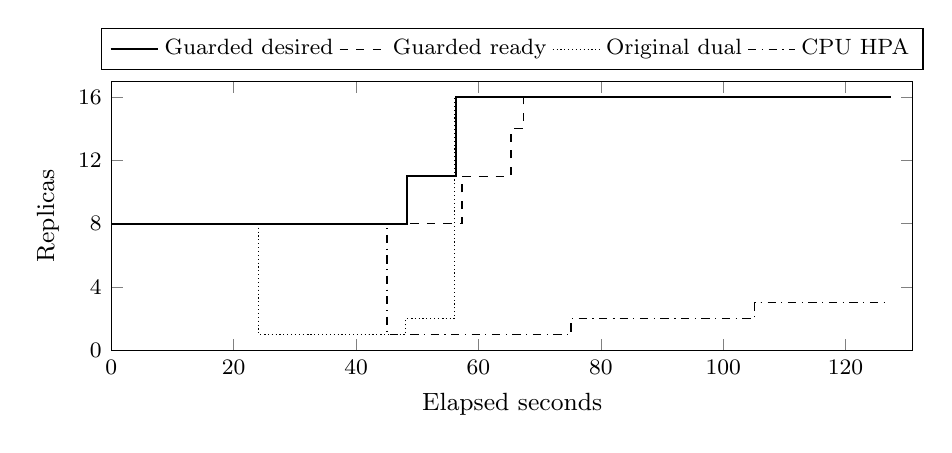
\begin{tikzpicture}\begin{axis}[width=.97\textwidth,height=5cm,xlabel={Elapsed seconds},ylabel={Replicas},xmin=0,xmax=131,ymin=0,ymax=17,ytick={0,4,8,12,16},legend style={at={(.5,1.04)},anchor=south,legend columns=4,font=\footnotesize},tick label style={font=\footnotesize},label style={font=\small}]
\addplot[const plot,no marks,black,thick] coordinates {(0.000,8) (1.001,8) (2.002,8) (3.004,8) (4.004,8) (5.005,8) (6.007,8) (7.009,8) (8.010,8) (9.011,8) (10.011,8) (11.012,8) (12.013,8) (13.014,8) (14.015,8) (15.017,8) (16.017,8) (17.018,8) (18.019,8) (19.021,8) (20.021,8) (21.023,8) (22.025,8) (23.027,8) (24.027,8) (25.028,8) (26.029,8) (27.030,8) (28.032,8) (29.033,8) (30.036,8) (31.037,8) (32.066,8) (33.066,8) (34.067,8) (35.068,8) (36.069,8) (37.070,8) (38.071,8) (39.074,8) (40.089,8) (41.089,8) (42.090,8) (43.090,8) (44.091,8) (45.092,8) (46.093,8) (47.095,8) (48.283,11) (49.284,11) (50.287,11) (51.287,11) (52.288,11) (53.290,11) (54.292,11) (55.294,11) (56.306,16) (57.307,16) (58.308,16) (59.310,16) (60.312,16) (61.313,16) (62.316,16) (63.317,16) (64.318,16) (65.319,16) (66.320,16) (67.320,16) (68.321,16) (69.323,16) (70.325,16) (71.327,16) (72.328,16) (73.330,16) (74.331,16) (75.331,16) (76.332,16) (77.333,16) (78.336,16) (79.337,16) (80.338,16) (81.340,16) (82.340,16) (83.341,16) (84.342,16) (85.343,16) (86.345,16) (87.347,16) (88.349,16) (89.351,16) (90.352,16) (91.353,16) (92.353,16) (93.354,16) (94.356,16) (95.358,16) (96.358,16) (97.359,16) (98.360,16) (99.361,16) (100.363,16) (101.365,16) (102.367,16) (103.369,16) (104.370,16) (105.370,16) (106.372,16) (107.372,16) (108.373,16) (109.374,16) (110.376,16) (111.379,16) (112.380,16) (113.381,16) (114.382,16) (115.383,16) (116.384,16) (117.385,16) (118.386,16) (119.388,16) (120.388,16) (121.389,16) (122.390,16) (123.390,16) (124.392,16) (125.393,16) (126.394,16) (127.396,16)};
\addlegendentry{Guarded desired}
\addplot[const plot,no marks,black,dashed] coordinates {(0.000,8) (1.001,8) (2.002,8) (3.004,8) (4.004,8) (5.005,8) (6.007,8) (7.009,8) (8.010,8) (9.011,8) (10.011,8) (11.012,8) (12.013,8) (13.014,8) (14.015,8) (15.017,8) (16.017,8) (17.018,8) (18.019,8) (19.021,8) (20.021,8) (21.023,8) (22.025,8) (23.027,8) (24.027,8) (25.028,8) (26.029,8) (27.030,8) (28.032,8) (29.033,8) (30.036,8) (31.037,8) (32.066,8) (33.066,8) (34.067,8) (35.068,8) (36.069,8) (37.070,8) (38.071,8) (39.074,8) (40.089,8) (41.089,8) (42.090,8) (43.090,8) (44.091,8) (45.092,8) (46.093,8) (47.095,8) (48.283,8) (49.284,8) (50.287,8) (51.287,8) (52.288,8) (53.290,8) (54.292,8) (55.294,8) (56.306,8) (57.307,11) (58.308,11) (59.310,11) (60.312,11) (61.313,11) (62.316,11) (63.317,11) (64.318,11) (65.319,14) (66.320,14) (67.320,16) (68.321,16) (69.323,16) (70.325,16) (71.327,16) (72.328,16) (73.330,16) (74.331,16) (75.331,16) (76.332,16) (77.333,16) (78.336,16) (79.337,16) (80.338,16) (81.340,16) (82.340,16) (83.341,16) (84.342,16) (85.343,16) (86.345,16) (87.347,16) (88.349,16) (89.351,16) (90.352,16) (91.353,16) (92.353,16) (93.354,16) (94.356,16) (95.358,16) (96.358,16) (97.359,16) (98.360,16) (99.361,16) (100.363,16) (101.365,16) (102.367,16) (103.369,16) (104.370,16) (105.370,16) (106.372,16) (107.372,16) (108.373,16) (109.374,16) (110.376,16) (111.379,16) (112.380,16) (113.381,16) (114.382,16) (115.383,16) (116.384,16) (117.385,16) (118.386,16) (119.388,16) (120.388,16) (121.389,16) (122.390,16) (123.390,16) (124.392,16) (125.393,16) (126.394,16) (127.396,16)};
\addlegendentry{Guarded ready}
\addplot[const plot,no marks,black,densely dotted] coordinates {(0.000,8) (1.002,8) (2.003,8) (3.004,8) (4.005,8) (5.006,8) (6.008,8) (7.011,8) (8.023,8) (9.023,8) (10.025,8) (11.025,8) (12.026,8) (13.027,8) (14.029,8) (15.030,8) (16.031,8) (17.032,8) (18.034,8) (19.036,8) (20.037,8) (21.039,8) (22.040,8) (23.042,8) (24.043,1) (25.043,1) (26.044,1) (27.045,1) (28.046,1) (29.047,1) (30.048,1) (31.051,1) (32.066,1) (33.066,1) (34.066,1) (35.067,1) (36.068,1) (37.070,1) (38.071,1) (39.072,1) (40.072,1) (41.074,1) (42.074,1) (43.075,1) (44.075,1) (45.076,1) (46.077,1) (47.079,1) (48.125,2) (49.125,2) (50.126,2) (51.126,2) (52.127,2) (53.128,2) (54.128,2) (55.130,2) (56.132,16) (57.133,16) (58.138,16) (59.140,16) (60.142,16) (61.142,16) (62.143,16) (63.145,16) (64.148,16) (65.149,16) (66.149,16) (67.150,16) (68.152,16) (69.153,16) (70.155,16) (71.156,16) (72.157,16) (73.158,16) (74.158,16) (75.159,16) (76.159,16) (77.160,16) (78.162,16) (79.164,16) (80.165,16) (81.166,16) (82.166,16) (83.167,16) (84.168,16) (85.169,16) (86.172,16) (87.174,16) (88.175,16) (89.177,16) (90.178,16) (91.179,16) (92.180,16) (93.181,16) (94.182,16) (95.184,16) (96.185,16) (97.187,16) (98.188,16) (99.188,16) (100.189,16) (101.190,16) (102.193,16) (103.196,16) (104.196,16) (105.197,16) (106.199,16) (107.200,16) (108.200,16) (109.201,16) (110.204,16) (111.207,16) (112.208,16) (113.209,16) (114.211,16) (115.212,16) (116.212,16) (117.213,16) (118.215,16) (119.216,16) (120.216,16) (121.216,16) (122.218,16) (123.218,16) (124.219,16) (125.220,16) (126.223,16) (127.225,16)};
\addlegendentry{Original dual}
\addplot[const plot,no marks,black,dashdotted] coordinates {(0.000,8) (1.001,8) (2.001,8) (3.002,8) (4.003,8) (5.004,8) (6.006,8) (7.007,8) (8.007,8) (9.008,8) (10.009,8) (11.010,8) (12.010,8) (13.011,8) (14.013,8) (15.015,8) (16.015,8) (17.017,8) (18.018,8) (19.018,8) (20.019,8) (21.021,8) (22.023,8) (23.026,8) (24.027,8) (25.027,8) (26.028,8) (27.029,8) (28.032,8) (29.032,8) (30.033,8) (31.035,8) (32.036,8) (33.038,8) (34.038,8) (35.039,8) (36.040,8) (37.041,8) (38.043,8) (39.044,8) (40.045,8) (41.046,8) (42.047,8) (43.048,8) (44.048,8) (45.049,1) (46.052,1) (47.055,1) (48.055,1) (49.056,1) (50.059,1) (51.059,1) (52.060,1) (53.061,1) (54.062,1) (55.063,1) (56.104,1) (57.105,1) (58.106,1) (59.106,1) (60.107,1) (61.108,1) (62.109,1) (63.110,1) (64.112,1) (65.113,1) (66.113,1) (67.117,1) (68.119,1) (69.120,1) (70.121,1) (71.123,1) (72.124,1) (73.125,1) (74.125,1) (75.128,2) (76.128,2) (77.129,2) (78.130,2) (79.131,2) (80.132,2) (81.132,2) (82.134,2) (83.135,2) (84.136,2) (85.137,2) (86.138,2) (87.140,2) (88.141,2) (89.143,2) (90.144,2) (91.144,2) (92.145,2) (93.146,2) (94.147,2) (95.150,2) (96.155,2) (97.156,2) (98.156,2) (99.158,2) (100.159,2) (101.160,2) (102.161,2) (103.163,2) (104.163,2) (105.164,3) (106.165,3) (107.166,3) (108.167,3) (109.168,3) (110.169,3) (111.170,3) (112.172,3) (113.173,3) (114.174,3) (115.175,3) (116.176,3) (117.178,3) (118.180,3) (119.181,3) (120.183,3) (121.184,3) (122.184,3) (123.185,3) (124.186,3) (125.188,3) (126.190,3) (127.192,3)};
\addlegendentry{CPU HPA}
\end{axis}\end{tikzpicture}\caption{Independent one-second replica observations from the predeclared first seed and previously used batch pattern. Desired capacity and ready capacity differ during actuation. All five repetitions enter the results; this trajectory is not selected for best SLO performance.}\label{fig:trajectory}\end{figure*}

\subsection{Allocation and Paired Comparisons}

\begin{table*}[t]\centering\small\setlength{\tabcolsep}{3pt}
\caption{Paired comparisons by workload and seed. Negative values indicate fewer violations or fewer desired pod-minutes for guarded control. All policies share a ceiling of sixteen replicas.}\label{tab:paired}
\savebox{\databox}{%
\begin{tabular}{llrrr}\toprule
Workload & Reference & Bad-rate difference pp & Paired 95\% interval & Allocation change \%\\\midrule
Previous batch & Original dual & -7.41 & [-11.84, -3.09] & 31.60\\
Previous batch & CPU HPA & -50.96 & [-58.94, -45.93] & 198.48\\
Previous batch & Fixed sixteen & 0.00 & [0.00, 0.00] & -22.40\\
Abrupt batch & Original dual & -31.39 & [-32.58, -30.01] & 32.10\\
Abrupt batch & CPU HPA & -31.50 & [-38.56, -24.44] & 218.83\\
Abrupt batch & Fixed sixteen & 0.00 & [0.00, 0.00] & -15.80\\
Continuous & Original dual & -20.67 & [-23.31, -16.62] & 7.22\\
Continuous & CPU HPA & -12.48 & [-23.98, -3.23] & 144.97\\
Continuous & Fixed sixteen & 0.00 & [0.00, 0.00] & -16.06\\
\bottomrule\end{tabular}
}
\ifdim\wd\databox>\textwidth\relax\resizebox{\textwidth}{!}{\usebox{\databox}}\else\usebox{\databox}\fi
\end{table*}

Mean desired allocation is 27.99 pod-minutes for guarded control, 22.90 for the original dual policy and 34.18 for fixed sixteen. Guarded allocation is 18.09\% below fixed sixteen on this trial measure, but exceeds that of the original dual policy, which frequently missed the objective. Thus the lower violation rate has a resource cost relative to that comparator. These figures cover the measured intervals; they exclude setup, warm-up and the cost of keeping reserves idle outside a trial.

\subsection{Reserve-Matched Native HPA}

\begin{table*}[t]\centering\small\setlength{\tabcolsep}{3pt}
\caption{Separate exploratory cohort with both adaptive policies initialized at eight and constrained to the same minimum eight and maximum sixteen. Three fresh paired repeats per workload; the frozen primary cohort is unchanged.}\label{tab:reserve_hpa}
\savebox{\databox}{%
\begin{tabular}{lrrrrrr}\toprule
Workload & Guarded met & HPA-eight met & Guarded bad \% & HPA-eight bad \% & Guarded pod-min & HPA-eight pod-min\\\midrule
Previous batch & 3/3 & 3/3 & 0.00 & 0.00 & 26.24 & 17.09\\
Abrupt batch & 3/3 & 3/3 & 0.00 & 0.00 & 28.83 & 17.08\\
Continuous & 3/3 & 3/3 & 0.00 & 0.00 & 29.15 & 17.09\\
\bottomrule\end{tabular}
}
\ifdim\wd\databox>\textwidth\relax\resizebox{\textwidth}{!}{\usebox{\databox}}\else\usebox{\databox}\fi
\end{table*}

Both policies met the SLO in all nine matched cells, with zero violations across 28,866 requests. Guarded control averaged 28.07 desired pod-minutes and HPA averaged 17.09. The allocation difference favoured HPA in each workload (Table~\ref{tab:reserve_hpa}). The higher minimum was sufficient for HPA in the follow-up. Because this cohort used different seeds, it provides a matched comparison under the higher minimum and leaves the effect of changing the minimum within the primary cohort unmeasured.

\subsection{Ablation and Stress Sensitivity}

\begin{table}[t]\centering\small\setlength{\tabcolsep}{3pt}
\caption{Live reserve ablation: guarded minus otherwise identical policy without the eight-replica floor. Both begin with eight ready replicas.}\label{tab:ablation}
\savebox{\databox}{%
\begin{tabular}{lrrr}\toprule
Workload & $\Delta$ bad pp & 95\% interval & $\Delta$ cost \%\\\midrule
Previous batch & 0.00 & [0.00, 0.00] & 2.53\\
Abrupt batch & -0.11 & [-0.18, -0.03] & 1.24\\
Continuous & -0.01 & [-0.03, 0.00] & -0.90\\
\bottomrule\end{tabular}
}
\ifdim\wd\databox>\columnwidth\relax\resizebox{\columnwidth}{!}{\usebox{\databox}}\else\usebox{\databox}\fi
\end{table}

Removing the eight-replica floor did not cause any trial to fail the 99\% objective. It did produce small nonzero violation fractions in the abrupt and continuous workloads. The guarded floor reduced the abrupt-workload mean by 0.11 percentage points at a 1.24\% allocation increase. For continuous traffic, guarded allocation was 0.90\% lower in the recorded runs, so these data do not support a uniform cost penalty or benefit from the floor.

\begin{table*}[t]\centering\small\setlength{\tabcolsep}{3pt}
\caption{Independent-plant means across 25 paired seeds per regime. All ablation columns show violation percentages. The central queue omits Kubernetes routing and CFS details, so these values are not live-cluster outcomes. Full eight-policy scores are retained in the artifact.}\label{tab:simulation}
\savebox{\databox}{%
\begin{tabular}{lrrrrrr}\toprule
Regime & Guarded & No reserve & No emergency & $h=1$ & CPU proxy & Guarded $n$\\\midrule
smooth & 0.00 & 0.00 & 0.00 & 0.00 & 0.00 & 13.26\\
burst & 0.00 & 0.00 & 0.00 & 0.00 & 1.04 & 15.36\\
service drift & 0.01 & 0.01 & 0.01 & 0.01 & 1.04 & 15.36\\
slow readiness & 0.00 & 0.00 & 0.00 & 0.00 & 4.44 & 15.35\\
observation delay & 0.00 & 0.00 & 0.00 & 0.00 & 2.17 & 15.32\\
\bottomrule\end{tabular}
}
\ifdim\wd\databox>\textwidth\relax\resizebox{\textwidth}{!}{\usebox{\databox}}\else\usebox{\databox}\fi
\end{table*}

The 1000 rollouts supplement the preserved 350-rollout pilot. In Table~\ref{tab:simulation}, removing emergency response or reducing the horizon to one produces the same displayed mean violation percentages as guarded control in all five regimes. At this precision, these ablations supply no clear evidence that either component improved compliance in the selected plant. The equality is specific to the simulated plant and reporting precision. A central dispatcher routes jobs to ready servers in the model, and the CPU proxy follows its own rule. Kubernetes routing, CFS throttling and native HPA reconciliation could change these outcomes.



\section{Discussion and Limitations}
\textbf{Pilot and primary capacity settings.} The pilot starts at one replica and can request up to six. In the primary study the adaptive policies begin at eight ready replicas and can request sixteen. We therefore use the rerun of the original dual policy under the larger ceiling when comparing it with the revision. That comparison measures the combined effect of the revised profile and control rules. The reserve and simulation ablations address individual rules under their own conditions.

\textbf{Interpreting the HPA comparison.} Native HPA could scale down to one in the primary study. When we gave it the same eight-replica floor as guarded control, both policies met the SLO in all nine matched cases. HPA averaged 17.09 desired pod-minutes and guarded control averaged 28.07. This is a direct comparison at the common floor on the three tested workloads. Because we specified the follow-up after seeing early primary outcomes and ran it with new seeds, it does not estimate the effect of changing the floor within the primary runs.

\textbf{Role of the response model.} The sizing equation uses the capacity threshold. The isotonic model estimates tail latency at the proposed count for diagnostics. In the eighteen validation blocks, we measured the CPU cost in the block where we recorded latency. The 94.04-ms effective-P99 mean absolute error therefore describes conditional response estimation. To test counterfactual decisions, we would also need evidence about the latency reached at alternative replica counts when CPU cost must be estimated before acting.

\textbf{Finite calibration and short trials.} The demand correction uses at most forty errors and caps its nominal-99\% rank at the largest observed score. It therefore has no exact distribution-free 99\% coverage guarantee. The capacity profile also consists of twenty short development blocks; their P99 estimates are especially uncertain at low request rates. The 200 CPU-ms/s cap, twenty-percent headroom, two extra replicas and pressure thresholds are engineering settings. Five primary repetitions per workload and three follow-up repetitions cannot establish a rare-event failure rate. Bootstrap intervals resample runs, and an interval of zero to zero only reflects the observed all-zero sample.

\textbf{Transfer to other deployments.} The Kubernetes measurements use generated traffic against one instrumented CPU endpoint on a shared laptop under WSL. HPA and the external controller retain different sensing and reconciliation timings. Two workload shapes contain drain intervals, while the third offers uninterrupted traffic. Longer runs, other services and other machines may change the balance between reserve cost and protection. Desired pod-minutes include requested capacity that is still pending, but exclude setup, warm-up and full-day idle allocation. They measure neither a cloud bill nor energy use. The simulator's central dispatcher and simplified CPU service omit routing and throttling effects present in Kubernetes, which limits transfer of its ablation findings.

The clearest remaining test is a live comparison across replica floors and startup delays, with the same initial conditions for both policies. That would show whether the extra capacity requested by the controller pays off when pods take longer to become ready.

\section{Conclusion}
With causal alignment, training-only scaling and gap filtering, the Prophet--LSTM hybrid beat persistence on NASA and trailed it on WorldCup. The live controller used a different predictor, based on recent request counts, and sized replicas from a profile of the CPU-bound service.

Across 75 primary trials and 120275 requests, the capacity-calibrated revision met the strict request objective in all fifteen workload--seed cells, compared with none for the original dual policy. It used 27.99 mean desired pod-minutes, below the 34.18 of fixed sixteen-replica capacity. In the eighteen-trial follow-up, HPA with a minimum of eight replicas met the objective in every cell and used fewer pod-minutes than the revision. The response checks describe this service at measured CPU costs, and the 1,000 simulation rollouts document stress behaviour under a separate queueing model. On the tested cluster, the revision fixed failures of the original controller. Whether it offers a benefit over native HPA at the same reserve remains open.

\appendix
\section{Reproducibility}
The public artifact contains the forecasting source snapshot and inputs, saved predictions, development profiles, live request traces, replica samples and frozen experiment protocols. The primary protocol records the seeds, workload schedules, controller settings and source hashes. The reserve-matched cohort has its own protocol because it was added later.

From \texttt{revision-20261114/}, \texttt{analyze.py} recomputes primary request counts, HTTP failures, latency statistics and timing checks. \texttt{analyze\_followup.py} audits the separate reserve-matched cohort. \texttt{verify\_simulation.py} checks shared generated inputs and replays two selected rollouts. Its saved verification also checks the simulation serialization repair against the original script hash. These commands check the archived evidence. To collect new primary observations, run \texttt{experiments.py} on a configured cluster.

The recorded environment is local K3s under Ubuntu WSL2. Dependency versions, application resources and an image digest are retained in \texttt{environment.json} and the environment notes. Infrastructure paths and the local API proxy must be adapted on another machine. The allocation audit checks the integral of sampled replicas and bounds the final unarchived partial interval; it cannot independently recover that exact terminal clock. The historical \texttt{build\_paper.py} generates an earlier draft and should not overwrite the current manuscript.

The current article is maintained in one \texttt{main.tex} file. Its sections, references, tables and vector plots are embedded, with older TeX drafts kept in archive folders. The README identifies the current manuscript and distinguishes analysis replay from fresh live execution.

\begin{thebibliography}{33}
\bibitem{guruge} P.~B. Guruge and Y.~H.~P.~P. Priyadarshana, ``Time series forecasting-based Kubernetes autoscaling using Facebook Prophet and Long Short-Term Memory,'' \emph{Frontiers in Computer Science}, vol.~7, article~1509165, 2025. \url{https://doi.org/10.3389/fcomp.2025.1509165}.
\bibitem{prophet} S.~J. Taylor and B.~Letham, ``Forecasting at Scale,'' \emph{The American Statistician}, 72(1), pp.~37--45, 2018. \url{https://doi.org/10.1080/00031305.2017.1380080}.
\bibitem{lstm} S.~Hochreiter and J.~Schmidhuber, ``Long Short-Term Memory,'' \emph{Neural Computation}, 9(8), pp.~1735--1780, 1997. \url{https://doi.org/10.1162/neco.1997.9.8.1735}.
\bibitem{bootstrap} B.~Efron, ``Bootstrap Methods: Another Look at the Jackknife,'' \emph{The Annals of Statistics}, 7(1), pp.~1--26, 1979. \url{https://doi.org/10.1214/aos/1176344552}.
\bibitem{j01} T.T.~Nguyen, Y.J.~Yeom, T.~Kim, D.H.~Park, S.~Kim, ``Horizontal Pod Autoscaling in Kubernetes for Elastic Container Orchestration,'' \emph{Sensors}, vol.~20, no.~16, pp.~4621, 2020. \url{https://doi.org/10.3390/s20164621}.
\bibitem{j02} D.R.~Augustyn, U.~Wycislik, M.~Sojka, ``Tuning a Kubernetes Horizontal Pod Autoscaler for Meeting Performance and Load Demands in Cloud Deployments,'' \emph{Applied Sciences}, vol.~14, no.~2, pp.~646, 2024. \url{https://doi.org/10.3390/app14020646}.
\bibitem{j03} S.K.~Mondal, X.~Wu, H.M.D.~Kabir, H.N.~Dai, K.~Ni, et al., ``Toward Optimal Load Prediction and Customizable Autoscaling Scheme for Kubernetes,'' \emph{Mathematics}, vol.~11, no.~12, pp.~2675, 2023. \url{https://doi.org/10.3390/math11122675}.
\bibitem{j04} O.~Pozdniakova, D.~Mazeika, A.~Cholomskis, ``SLA-Adaptive Threshold Adjustment for a Kubernetes Horizontal Pod Autoscaler,'' \emph{Electronics}, vol.~13, no.~7, pp.~1242, 2024. \url{https://doi.org/10.3390/electronics13071242}.
\bibitem{j05} J.~Dogani, F.~Khunjush, M.~Seydali, ``K-AGRUED: A Container Autoscaling Technique for Cloud-based Web Applications in Kubernetes Using Attention-based GRU Encoder-Decoder,'' \emph{Journal of Grid Computing}, vol.~20, no.~4, article~40, 2022. \url{https://doi.org/10.1007/s10723-022-09634-x}.
\bibitem{j06} J.~Dogani, R.~Namvar, F.~Khunjush, ``Auto-scaling techniques in container-based cloud and edge/fog computing: Taxonomy and survey,'' \emph{Computer Communications}, vol.~209, pp.~120--150, 2023. \url{https://doi.org/10.1016/j.comcom.2023.06.010}.
\bibitem{j07} X.~Feng, S.~Zhang, T.~Jiao, C.~Guo, J.~Song, ``Adaptive container auto-scaling for fluctuating workloads in cloud,'' \emph{Future Generation Computer Systems}, vol.~172, pp.~107872, 2025. \url{https://doi.org/10.1016/j.future.2025.107872}.
\bibitem{j08} S.~Alharthi, A.~Alshamsi, A.~Alseiari, A.~Alwarafy, ``Auto-Scaling Techniques in Cloud Computing: Issues and Research Directions,'' \emph{Sensors}, vol.~24, no.~17, pp.~5551, 2024. \url{https://doi.org/10.3390/s24175551}.
\bibitem{j09} S.~Verma, A.~Bala, ``Auto-scaling techniques for IoT-based cloud applications: a review,'' \emph{Cluster Computing}, vol.~24, no.~3, pp.~2425--2459, 2021. \url{https://doi.org/10.1007/s10586-021-03265-9}.
\bibitem{j10} J.~Herrera, G.~Molto, ``Toward Bio-Inspired Auto-Scaling Algorithms: An Elasticity Approach for Container Orchestration Platforms,'' \emph{IEEE Access}, vol.~8, pp.~52139--52150, 2020. \url{https://doi.org/10.1109/access.2020.2980852}.
\bibitem{j11} Y.~Guo, A.~L. Stolyar, and A.~Walid, ``Online VM Auto-Scaling Algorithms for Application Hosting in a Cloud,'' \emph{IEEE Transactions on Cloud Computing}, vol.~8, no.~3, pp.~889--898, 2020. \url{https://doi.org/10.1109/tcc.2018.2830793}.
\bibitem{j12} J.M.~Lopez, J.~Garcia, J.L.~Diaz, M.~Garcia, J.~Entrialgo, et al., ``Techniques for efficient resource allocation transitions in container cluster autoscaling,'' \emph{Journal of Cloud Computing}, 2026. \url{https://doi.org/10.1186/s13677-026-00970-x}.
\bibitem{j13} B.~Kumar, A.~Verma, P.~Verma, A.~Bennour, ``Optimizing resource allocation in cloud-native applications through proactive autoscaling with the InformerAutoScale model,'' \emph{The Journal of Supercomputing}, vol.~81, no.~9, article~1077, 2025. \url{https://doi.org/10.1007/s11227-025-07500-7}.
\bibitem{j14} D.~Saxena, A.K.~Singh, ``A proactive autoscaling and energy-efficient VM allocation framework using online multi-resource neural network for cloud data center,'' \emph{Neurocomputing}, vol.~426, pp.~248--264, 2021. \url{https://doi.org/10.1016/j.neucom.2020.08.076}.
\bibitem{j15} B.~Kumar, A.~Verma, P.~Verma, ``A multivariate transformer-based monitor-analyze-plan-execute (MAPE) autoscaling framework for dynamic resource allocation in cloud environment,'' \emph{Computing}, vol.~107, no.~3, article~69, 2025. \url{https://doi.org/10.1007/s00607-025-01426-x}.
\bibitem{j16} I.K.~Kim, W.~Wang, Y.~Qi, M.~Humphrey, ``Forecasting Cloud Application Workloads With CloudInsight for Predictive Resource Management,'' \emph{IEEE Transactions on Cloud Computing}, vol.~10, no.~3, pp.~1848--1863, 2022. \url{https://doi.org/10.1109/tcc.2020.2998017}.
\bibitem{j17} G.~Quattrocchi, E.~Incerto, R.~Pinciroli, C.~Trubiani, L.~Baresi, ``Autoscaling Solutions for Cloud Applications Under Dynamic Workloads,'' \emph{IEEE Transactions on Services Computing}, vol.~17, no.~3, pp.~804--820, 2024. \url{https://doi.org/10.1109/tsc.2024.3354062}.
\bibitem{j18} N.M.~Dang-Quang, M.~Yoo, ``Deep Learning-Based Autoscaling Using Bidirectional Long Short-Term Memory for Kubernetes,'' \emph{Applied Sciences}, vol.~11, no.~9, pp.~3835, 2021. \url{https://doi.org/10.3390/app11093835}.
\bibitem{j19} K.M.~Alam, A.~El Saddik, ``C2PS: A Digital Twin Architecture Reference Model for the Cloud-Based Cyber-Physical Systems,'' \emph{IEEE Access}, vol.~5, pp.~2050--2062, 2017. \url{https://doi.org/10.1109/access.2017.2657006}.
\bibitem{j20} Q.~Yu, Z.~Cao, R.~Wang, Z.~Yang, L.~Deng, et al., ``Dual-splitting conformal prediction for multi-step time series forecasting,'' \emph{Applied Soft Computing}, vol.~184, pp.~113825, 2025. \url{https://doi.org/10.1016/j.asoc.2025.113825}.
\bibitem{j21} F.~Schlembach, E.~Smirnov, I.~Koprinska, M.H.M.~Winands, ``Conformal multistep-ahead multivariate time-series forecasting,'' \emph{Machine Learning}, vol.~114, no.~7, article~165, 2025. \url{https://doi.org/10.1007/s10994-024-06722-9}.
\bibitem{j22} M.~Smendowski, P.~Nawrocki, ``Optimizing multi-time series forecasting for enhanced cloud resource utilization based on machine learning,'' \emph{Knowledge-Based Systems}, vol.~304, pp.~112489, 2024. \url{https://doi.org/10.1016/j.knosys.2024.112489}.
\bibitem{j23} H.~Han, Z.~Liu, M.~Barrios Barrios, J.~Li, Z.~Zeng, et al., ``Time series forecasting model for non-stationary series pattern extraction using deep learning and GARCH modeling,'' \emph{Journal of Cloud Computing}, vol.~13, no.~1, article~2, 2024. \url{https://doi.org/10.1186/s13677-023-00576-7}.
\bibitem{j24} B.~Jeong, Y.S.~Jeong, ``Autoscaling techniques in cloud-native computing: A comprehensive survey,'' \emph{Computer Science Review}, vol.~58, pp.~100791, 2025. \url{https://doi.org/10.1016/j.cosrev.2025.100791}.
\bibitem{j25} B.~Jeong, J.~Jeon, Y.S.~Jeong, ``Proactive Resource Autoscaling Scheme Based on SCINet for High-Performance Cloud Computing,'' \emph{IEEE Transactions on Cloud Computing}, vol.~11, no.~4, pp.~3497--3509, 2023. \url{https://doi.org/10.1109/tcc.2023.3292378}.
\bibitem{j26} S.~Singh, I.~Chana, ``Cloud resource provisioning: survey, status and future research directions,'' \emph{Knowledge and Information Systems}, vol.~49, no.~3, pp.~1005--1069, 2016. \url{https://doi.org/10.1007/s10115-016-0922-3}.
\bibitem{j27} S.N.A.~Jawaddi, M.H.~Johari, A.~Ismail, ``A review of microservices autoscaling with formal verification perspective,'' \emph{Software: Practice and Experience}, vol.~52, no.~11, pp.~2476--2495, 2022. \url{https://doi.org/10.1002/spe.3135}.
\bibitem{j28} S.R.~Jeremiah, A.~El Azzaoui, N.N.~Xiong, J.H.~Park, ``A comprehensive survey of digital twins: Applications, technologies and security challenges,'' \emph{Journal of Systems Architecture}, vol.~151, pp.~103120, 2024. \url{https://doi.org/10.1016/j.sysarc.2024.103120}.
\bibitem{j29} F.~Agullo, A.~Gutierrez-Torre, J.~Torres, J.L.~Berral, ``Enhancing the output of time series forecasting algorithms for cloud resource provisioning,'' \emph{Future Generation Computer Systems}, vol.~170, pp.~107833, 2025. \url{https://doi.org/10.1016/j.future.2025.107833}.
\end{thebibliography}
\end{document}